\documentclass[12pt, oneside, titlepage]{article}   	% use "amsart" instead of "article" for AMSLaTeX format

\usepackage{graphicx}
\graphicspath{ {\string} }
\usepackage{subcaption}

%%%%%%%%%%%%%%%%%%%%%%%%%%%%%%%%%%%%%%%%%%%%%%%%%%%%
% set up packages
%%%%%%%%%%%%%%%%%%%%%%%%%%%%%%%%%%%%%%%%%%%%%%%%%%%%
\usepackage{geometry}                
\usepackage{textcomp}                
\usepackage{amsmath}                
\usepackage{graphicx}                
\usepackage{amssymb}                
\usepackage{fancyhdr}                
\usepackage{subcaption}                
\usepackage{bm}                
\usepackage{lineno}
% package for comments
\usepackage{soul}
\usepackage[usenames, dvipsnames]{color}

\usepackage[breaklinks=true]{hyperref}
\hypersetup{
    colorlinks=true,
    linkcolor=red,
    filecolor=orange,      
    urlcolor=red,
    citecolor=Violet,
}

\usepackage[superscript,noadjust]{cite} % puts dash in citations to abbreviate
\usepackage [autostyle, english = american]{csquotes} % sets US-style quotes

\usepackage{etoolbox} % block quotes

\usepackage{float}

\usepackage{pgf}
\usepackage{tikz}
\usepackage{eqnarray}

\usepackage{listings} % code blocks
\usepackage{setspace}

\usepackage{natbib}
%\bibliographystyle{abbrvnat}
\setcitestyle{authoryear}

% Adds parentheses around year
%\setcitestyle{authoryear,open={(},close={)}}

%%%%%%%%%%%%%%%%%%%%%%%%%%%%%%%%%%%%%%%%%%%%%%%%%%%%
% call packages
%%%%%%%%%%%%%%%%%%%%%%%%%%%%%%%%%%%%%%%%%%%%%%%%%%%%	
\geometry{letterpaper, marginparwidth=60pt} % sets up geometry              		
\linenumbers % adds line numbers 
\MakeOuterQuote{"} % sets quote style
\doublespacing % setspace

%%%%%%%%%%%%%%%%%%%%%%%%%%%%%%%%%%%%%%%%%%%%%%%%%%%%
% patches with etoolbox 
%%%%%%%%%%%%%%%%%%%%%%%%%%%%%%%%%%%%%%%%%%%%%%%%%%%%	

% linenumbers
\makeatletter
\patchcmd{\@startsection}{\@ifstar}{\nolinenumbers\@ifstar}{}{}
\patchcmd{\@xsect}{\ignorespaces}{\linenumbers\ignorespaces}{}{}
\makeatother

%%%%%%%%%%%%%%%%%%%%%%%%%%%%%%%%%%%%%%%%%%%%%%%%%%%%
% page formatting; exact 1 in margins
%%%%%%%%%%%%%%%%%%%%%%%%%%%%%%%%%%%%%%%%%%%%%%%%%%%%
\pagestyle{plain}                                                     

\setlength{\textwidth}{6.5in}    
\setlength{\oddsidemargin}{0in}
\setlength{\evensidemargin}{0in}
\setlength{\textheight}{8.5in}
\setlength{\topmargin}{0in}
\setlength{\headheight}{0in}
\setlength{\headsep}{0in}
\setlength{\footskip}{.5in}

%%%%%%%%%%%%%%%%%%%%%%%%%%%%%%%%%%%%%%%%%%%%%%%%%%%%
% TABLE OF CONTENTS TITLE
%%%%%%%%%%%%%%%%%%%%%%%%%%%%%%%%%%%%%%%%%%%%%%%%%%%%
\renewcommand{\contentsname}{Methods}
\setcounter{tocdepth}{3}

%%%%%%%%%%%%%%%%%%%%%%%%%%%%%%%%%%%%%%%%%%%%%%%%%%%%
%%%%%%%%%%%%%%%%%%%%%%%%%%%%%%%%%%%%%%%%%%%%%%%%%%%%
% begin document
%%%%%%%%%%%%%%%%%%%%%%%%%%%%%%%%%%%%%%%%%%%%%%%%%%%%
%%%%%%%%%%%%%%%%%%%%%%%%%%%%%%%%%%%%%%%%%%%%%%%%%%%%

\begin{document}

\tableofcontents

\clearpage
%%%%%%%%%%%%%%%%%%%%%%%%%%%%%%%%%%%%%%%%%%%%%%%%%%%%
% METHODS
%%%%%%%%%%%%%%%%%%%%%%%%%%%%%%%%%%%%%%%%%%%%%%%%%%%%
%\section\subsection{Methods}

\section{Background on study system}

Starting in 2006, Monica Geber and collaborators have collected 12+ years of annual estimates for demographic data on the winter annual plant \textit{Clarkia xantiana} ssp. \textit{xantiana}. The data include annual estimates for survival of seedlings to fruiting adults, fruits per adult plant, and seeds per fruit. In addition the data on above-ground vital rates, experiments have been used to infer germination and seed survival in the seed bank. The demographic study has been used to test hypotheses about the geography of demography (\cite{eckhart2011}) and species distributions (\cite{pironon2018}).

% Starting in 2007, there are (1) estimates of fruits/plant and seeds/fruit that provide an estimate of seed input into a plot and (2) estimates of germinants the following year. For most plots, the number of seeds entering a plot in year $t-1$ is much greater than the number of seedlings emerging in a plot in year $t$. However, this is not uniformly true, and there is also experimental data suggesting these seeds may survive in the seed bank for at least 10 years at some locations.

%We use two experiments, conducted at non-overlapping points in time, to estimate transitions in the seed bank. From 2006-2010, Geber and collaborators buried seeds in bags and periodically dug them up to count seedlings and intact, viable seeds. This data estimates transitions leading to germination or survival of seeds that are 1, 2, and 3 years old. Starting in 2013, Geber and collaborators placed seeds in pots and counted seedlings. This data estimates transitions of seeds in the soil seed bank but cannot separate germination and survival in the same way as the first experiment.

%\hl{To compare the data to Lewis 1963, we examine the presence/absence trajectories of permanent plots and population-level data. Both individual plot and abundance data suggest that locations within a population can not have any fruiting plants for several years and later recover in abundance. The most drastic example perhaps comes from Lucas Creek East, where there is a 4 year gap in which there are no plants in any of the permanent plots before abundance increases again. We take this as motivation to study the role of seed banks in maintaining populations through time.}

\section{Demographic modeling framework}

We use observational and experimental data from 20 populations of \textit{Clarkia xantiana} to estimate transition probabilities across the life cycle. We model population-specific estimates for belowground vital rates, and model year- and population-specific estimates for aboveground vital rates. We use these parameter estimates to analyze correlations between germination probability and variance in per-capita reproductive success, correlation between germination probability and seed survival, and to compare the observed germination fraction to the optimal germination fraction from a density-independent model. 

\subsection{Belowground transitions}

To estimate population-specific estimates for belowground vital rates, I use data from seed burial experiments in the field and seed viability trials in the lab. I combine these data to infer germination and seed survival. Briefly, I estimate probabilities of success using data from seed burial experiments and viability trials ($\theta_1, \theta_2, \theta_3, \theta_4, \theta_5, \theta_g, \theta_v$). I use these probabilities to compose transition probabilities that correspond to the life history of \textit{Clarkia xantiana}($s_1, s_2, s_3, g_1$). I describe this approach in detail in the \textbf{Appendix on Conditional Probability}. Figure~\ref{fig:seedBagDiagram} illustrates the relationship between the data and the estimated probability of success. 
 
The probability that seeds from the start of the experiment remain intact in January is represented as $\theta_1$. In January, all seeds are intact (this includes viable and non-viable seeds). I estimate the probability of a seedling emerging, conditional on being intact as $\theta_2$. I assume that there is no decay or loss of viability during germination. The number of intact seeds before germination is equal to the sum of the number of seeds and seedlings after germination. At this point, seeds transition into one of four possible states. Intact and viable seeds may have (1) germinated or (2) not germinated and remained dormant. All (3) other intact seeds are non-viable because (4) seeds that were not viable could not have germinated. Finally, we represent the probability of a seed being intact in October, conditional on being intact in January as $\theta_3$.

% I represent two transitions between pre-germination seeds in January and post-germination seeds and seedlings in January. The first is for seeds that are viable and germinate; these become seedlings. The second is for seeds that do not germinate; these remain seeds and include both viable and non-viable seeds. For the purposes of parameter estimation, I only represent the number of seedlings\textemdash viability is estimated separately. 

We use the viability trials to estimate the probability of viability ($\nu_1$) for a seed that is intact in October one year after the seed bags were buried. The viability trials are a two-stage process: seeds are subject to germination trials before a fraction of the remaining, ungerminated seeds are tested for viability. The probability that a seed germinates in the germination trial is $\theta_g$ and the probability that it is viable, conditional on not germinating in the germination trial, is $\theta_v$. I estimate the overall probability of viability, $\nu$, as $\theta_g + \theta_v (1-\theta_g)$. This weights the estimates relative to the probability of germination (eg. if no seeds germinate the estimate of viability will mostly come from the viability test).

I make some assumptions in order to incorporate the loss of viability into the model. I assume that viability is lost at a constant rate, and that germination removes some number of seeds from the pool of viable seeds but does not change the rate of decay. Some fraction of the intact seeds in January are viable before germination ($\nu_1^{1/3}$), and some of those viable seeds germinate. 

The seed burial experiments and viability trials provide information about the fate of seeds in the seed bank. We define $s_1$ as the probability of a seed being intact and viable from October in year $t$ to January in year $t+1$. We define $g_1$ as the probability of germination for a seed that is intact and viable. We define $s_2$ as the probability of survival from January to October in year $t$ for a seed that was intact and viable in January.  Mathematically, we write each of the transition probabilities as follows:
%
    \begin{align}
\begin{split}
s_1 & = \theta_1 \times (\theta_2 + ( 1- \theta_2 ) \times \nu_1^{1/3} ) \\
g_1 & = \frac{\theta_2 }{1 - ( 1-  \nu_1^{1/3} ) \times ( 1 - \theta_2 )} \\
s_2 & = \theta_3 \times \nu_1^{2/3} \\
  \end{split}
\end{align}
%
To estimate the survival of two-year old seeds from October to January ($s_3$) requires some additional assumptions. First, we used a different set of bags for these estimates than for the estimates of first-year rates ($s_1, s_2, g_1$). We use the second set of bags to estimate the probability of viability ($\nu_2$) as described above, combining $\theta_g$ and $\theta_v$. We calculate the viability in the second January as the product of viability at the end of the first year ($\nu_1$) and the fraction of first year viability remaining in January ($ (\nu_2 \div \nu_1)^{1/3} $). For cases where $\nu_2 \geq \nu_1$, we assumed that all seeds in the bag were viable in October $t+1$ and calculated the fraction of first year viability remaining in January as $ (\nu_2 )^{1/3} $.

When I estimate the probability of seedling survival from the second October to second January ($s_3$), I incorporate the expected proportion of seeds that are expected to be intact at the end of the first year ($\theta_1(1-\theta_2) \theta_3$). I define $s_3$ as the probability of survival from October in year $t$ to January in year $t+1$ for a seed that was intact and viable in October. Mathematically, we write the transition probability as follows:
%
    \begin{align}
\begin{split}
s_3 & = \theta_4 \times (\theta_5 + ( 1- \theta_5 ) \times \nu_2^{1/3} )
  \end{split}
\end{align}
%
\subsection{Aboveground transitions}

To obtain year- and population-specific estimates for aboveground vital rates, we use data from annual observational surveys of 20 \textit{Clarkia xantiana} populations. We use data from surveys of plots to estimate seedling survival to fruiting ($\phi$). We also estimate total fruit equivalents per plant ($F$) and seeds per fruit ($\phi$). We combine these data to obtain annual estimates of per-capita reproductive reproductive success.

From 2006--2012, we counted total fruit equivalents in the field, and estimated the number of seeds in undamaged fruits in the lab. Starting in 2013, we began to count undamaged and damaged fruits in the field, and estimate the number of seeds in both undamaged and damaged fruits in the lab. To compare these components of fitness across all years of the study, we converted the number of undamaged and damaged fruits to total fruit equivalents with the following relationship:
%
    \begin{align}
\begin{split}
\textrm{TFE} = \textrm{undamaged fruits} + \frac{\textrm{seeds per damaged fruit}}{\textrm{seeds per undamaged fruit}}\times  \textrm{damaged fruits} 
  \end{split}
\end{align}
%
In these calculations, we use the marginalized, posterior distributions from the models for fruits per plant and seeds per fruit. We use the number of seeds per undamaged fruit to calculate per-fruit seed production. While using a single measure for counts of fruits per plant might be ideal, such a metric is not available to us. We instead combine several sources of data to constrain our estimate while propagating uncertainty from those estimates. 

\section{Data}

\subsection{Seed survival and germination}

\subsubsection{Seed bag burial experiments}

To assess germination and seed survival throughout the year in \textit{C. xantiana}, we use data collected from a series of seed burial experiments. In June-July 2005, we collected seeds at each of the 20 populations included in this study. In October 2005, we buried 30 5$\times$5-cm nylon mesh bags at each population. Each nylon mesh bag contained 100 seeds collected at that population. In January 2006, we removed 10 of these bags and counted the number of germinated seedlings and the number of ungerminated, intact seeds in each bag. We then returned the ungerminated, intact seeds to the resealed bag and returned the bag to the field. In October 2006, we removed these bags and counted the number of ungerminated, intact seeds. We collected the following data:

\begin{itemize}
	\item $n_{ijt}$ = observed count of seeds in the seed bags at the start of the experiment in October in the $i^{th}$ bag, from the $j^{th}$ population, in the $t^{th}$ year, assumed to be measured perfectly 
	\item $y^{\mathrm{intact}}_{ijt}$ = observed count of ungerminated, intact seeds in the seed bags in January in the $i^{th}$ bag, from the $j^{th}$ population, in the $t^{th}$ year,  assumed to be measured perfectly 
	\item $y^{\mathrm{germ}}_{ijt}$ = observed count of germinated seedlings in the seed bags in January in the $i^{th}$ bag, from the $j^{th}$ population, in the $t^{th}$ year, assumed to be measured perfectly 
	\item $y^{\mathrm{total}}_{ijt}$= observed count of ungerminated, intact seeds plus germinated seedlings in the seed bags in January in the $i^{th}$ bag, from the $j^{th}$ population, in the $t^{th}$ year, assumed to be measured perfectly 	
	\item $y^{\mathrm{surv}}_{ijt}$ = observed count of ungerminated, intact seeds in the seed bags in October in the $i^{th}$ bag, from the $j^{th}$ population, in the $t^{th}$ year, assumed to be measured perfectly 	
\end{itemize}

We started these seed burial experiments in three subsequent years (2005, 2006, 2007) to obtain multiple estimates for seed survival and germination. 

\subsubsection{Viability trials}

To assess what proportion of intact seeds are viable, we use data collected from viability assays conducted on seeds when they are unearthed in October.  Only some proportion of the seeds that are unearthed intact in the seed burial experiments are likely to be viable--put another way, seeds that are intact may not be viable.Because seeds unearthed in January are reburied, we do not have direct estimates of viability in January.

Each year that we conducted seed burial experiments, we also conducted seed viability trials. After bags were removed from the field in October, we returned the bags to the lab. In the lab, we conducted germination trials and viability assays on subsets of the seeds from each bag to estimate the viability of the ungerminated, intact seeds. First, we placed up to 15 seeds from each bag on to moist filter paper in a disposable cup and observed germination over 10 days; we counted and removed germinants every 2 days. 

After 10 days, all remaining ungerminated seeds (up to a total of 10 seeds) were sliced in half and individually placed into the wells of 96-well plates filled with a solution of tetrazolium chloride, which stains viable tissue red. [\cite{eckhart2011}: \hl{not all ungerminated seeds were tested; most were}] We covered the plates with foil. Each 96-well plate contained seed from at least one bag per population of a given seed-age class. Two or three tests of up to 15 seeds each were conducted for each bag. We checked and counted for viable seeds every 2 days for 10 days. 

We collected the following data: 

\begin{itemize}
	\item $n^{\mathrm{germ}}_{ijt}$ = observed count of seeds at the start of the $X^{th}$ germination trial for the $i^{th}$ bag, from the $j^{th}$ population, in the $t^{th}$ year, assumed to be measured perfectly
	\item $y^{\mathrm{germ}}_{ijt}$ = observed count of germinated seedlings in the $X^{th}$ germination trial for the $i^{th}$ bag, from the $j^{th}$ population, in the $t^{th}$ year, assumed to be measured perfectly 
	\item $n^{\mathrm{viab}}_{ijt}$ = observed count of seeds at the start of the $X^{th}$ viability trial for the $i^{th}$ bag, from the $j^{th}$ population, in the $t^{th}$ year, assumed to be measured perfectly 
	\item $y^{\mathrm{viab}}_{ijt}$ = observed count of viable seedlings in the $X^{th}$ viability trial for the $i^{th}$ bag, from the $j^{th}$ population, in the $t^{th}$ year, assumed to be measured perfectly 
\end{itemize}

\subsection{Seedling survival to fruiting}

To assess the survival of germinants to fruiting plants for \textit{C. xantiana}, we use data of counts of seedlings and fruiting plants in 30 0.5 m$^2$ plots at 20 populations from 2006--present (\cite{eckhart2011}). Each population was visited in February and June to count the number of seedlings and fruiting plants, respectively. Seedlings and fruiting plants in each plot are counted by a single person at each visit. 

While we assume that the data on seedlings is measured perfectly (i.e. we did not under- or over-count seedlings), there are at least two possible sources of error: (1) measurement error that arises because we failed to count seedlings that were present and (2) error that arises because seedlings germinated after we visited the population. Germination phenology varies from year to year and with the position of the population in the range. \hl{For now, I ignore data that involved undercounting by filtering out those rows in the dataset. We may want to develop a model that relates our estimate of seedlings to the true number of seedlings in a plot because we sometimes observe more fruiting plants than seedlings but I had trouble developing such a model for the time being.}

We assume that the data on fruiting plants is measured perfectly (i.e. we did not under- or over-count) because plants stand out from the background vegetation in June. Our model estimates the proportion of seedlings that survive to become fruiting plants. Define:

\begin{itemize}
	\item $n_{ijk}$ = observed counts of seedlings in the $i^{th}$ plot, from the $j^{th}$ population, from the $k^{th}$ year
	%\item $z_{ijt}$ = true counts of seedlings in the $i^{th}$ plot, from the $j^{th}$ population, from the $t^{th}$ year
	\item $y_{ijk}$ = observed counts of fruiting plants in the $i^{th}$ plot, from the $j^{th}$ population, from the $k^{th}$ year, assumed to be measured perfectly
\end{itemize}

\subsection{Fruits per plant}

To assess the number of fruits per plant for \textit{C. xantiana}, we use data on counts of the number of fruits per plant at 20 populations (\cite{eckhart2011}). At each population, we made two sets of counts. First, we counted the number of fruits per plant on all plants in the 0.5m$^2$ permanent plots. Second, we counted the number of fruits per plant on plants that we sampled haphazardly across the site using throws of a 0.5m$^2$ grid.

From 2006--2012, we counted the number of undamaged fruits on a plant. We then took the damaged fruits on a plant and visually stacked them end to end to estimate how many additional undamaged fruits that was equivalent to (e.g. two half fruits corresponded to one undamaged fruit). We used these counts to estimate the number fruits produced per plant. 

From 2013--present, we counted the number of undamaged and damaged fruits on a plant plant. We used these counts to estimate the number of fruits produced per plant.

We seek to estimate the number of fruits produced per plant. Define: 

\begin{itemize}

	\item $y^{TFE}_{ijk}$ = observed counts of total fruit equivalents per plant on the $i^{th}$ plant, from the $j^{th}$ population, from the $k^{th}$ year, assumed to be measured perfectly
%	\item $\bm{y_{ijk}} = [ y^{und}_{ijt}, y^{dam}_{ijt} ] $ = two item vector of observed counts of undamaged and damaged fruits per plant on the $i^{th}$ plant, from the $j^{th}$ population, from the $k^{th}$ year, assumed to be measured perfectly
	\item $n_{ijk}$ = observed counts of total fruits per plant (sum of $\bm{y_{ijk}}$) on the $i^{th}$ plant, from the $j^{th}$ population, from the $k^{th}$ year, assumed to be measured perfectly
%	\item $\phi_{jt}$ = the true, unobserved proportion of fruits that are damaged per plant at the $j^{th}$ population, in the $k^{th}$ year
\end{itemize}

\subsection{Seeds per fruit}

To assess the number of seeds per fruit for \textit{C. xantiana}, we use data on counts of the seeds per fruit of fruits that were haphazardly collected in 20 populations (\cite{eckhart2011}). In the field, we collected fruits that were undamaged. In the lab, we broke open the fruits to count the number of seeds per fruit. For each population in each year, we attempted to obtain 20-30 counts of seeds produced per undamaged fruit. 

From 2006--2012, we collected one undamaged fruit from each of 20-30 plants that were haphazardly collected across each population.

From 2013--present, we collected one undamaged and one damaged fruit from each of 20-30 haphazardly selected plants distributed across each population. The plants were outside permanent plots to avoid affecting seed input. We used these fruits to estimate the mean number of seeds produced by undamaged and damaged fruits. In the lab, we broke open the fruits to count the number of seeds per fruit. For each population in each year, we attempted to obtain 20-30 counts of seeds produced per undamaged fruit and  20-30 counts of seeds produced per damaged fruit. 

We seek to estimate the number of seeds per undamaged fruit. Define:

\begin{itemize}
	\item $y^{und}_{ijk}$ = observed counts of seeds in the $i^{th}$ undamaged fruit, from the $j^{th}$ population, from the $k^{th}$ year, assumed to be measured perfectly
%	\item $y^{dam}_{ijt}$ = observed counts of seeds per damaged fruit in the $i^{th}$ fruit, from the $j^{th}$ population, from the $k^{th}$ year, assumed to be measured perfectly
	\item $\lambda_{jk}$ = true, unobserved mean number of seeds per undamaged fruit from the $j^{th}$ population, from the $k^{th}$ year
\end{itemize}

\section{Models for parameter estimates}

Across all datasets, we have data from multiple years and populations. The goal is to obtain model-based estimates of vital rates. We use the models to separate variability in parameters between temporal variability and variability due to sampling (e.g. \cite{gould1998}). This is particularly important for our estimates of per capita reproductive success because we calculate annual estimates to quantify interannual variation. Failing to account for sampling variation can inflate estimates of temporal variation. Sample sizes for parameters vary both within years across populations, as well as across populations. Accounting for sampling variability is important for making conclusions about differences among populations. 
 
\subsection{Seed survival and germination}

All data from seed bags and viability trials is in the form of binomial trials: we have counts of seeds at the start and end of an experimental window of time. All models have the same structure for seeds in bag $i$ in year $j$ in population $k$. If the number of seeds starting the trial (trials) is $n_{ijk}$ and the number of seeds at the end of the trial (successes) is $y_{ijk}$, we write a model that has a population-level mean and year-level means drawn from the population-level distribution. Broadly, this is two-level hierarchical model with a population-level mean, and year-level means drawn from the population-level distribution. The probability of success for each bag is drawn from this year- and population-level distribution. The model uses a binomial likelihood. The joint posterior for viability trials, seed bag experiments in the first year, and for germination of seeds in the second year thus has the following general form:
%
\begin{align}
  \begin{split}
 [  \bm{\alpha} , \bm{\mu} , \bm{\sigma} , \bm{\mu^\mathrm{pop}}, \bm{\sigma^\mathrm{pop}} | & \bm{y^{\mathrm{tot}}}  ] \propto \prod_{i=1}^{I}   \prod_{j=1}^{J}  \prod_{k=1}^{K} 
   \mathrm{binomial} ( y_{ijk} | n_{ijk}, \mathrm{logit}^{-1}( \alpha_{ijk} ) ) 
   \\ & \times \mathrm{normal} ( \alpha_{ijk}  | \mu_{jk}, \sigma{_{jk} })
  \\ & \times \mathrm{normal} ( \mu_{jk}  | \mu^\mathrm{pop}_{j}, \sigma^\mathrm{pop}_{j} )
  \\ & \times \textrm{half-normal} ( \sigma_{jk} | 0,1)
  \\ & \times \mathrm{normal} ( \mu^\mathrm{pop}_{j} | 0 , 1000 ) \textrm{half-normal} ( \sigma^\mathrm{pop}_{j} | 0,1).
  \end{split}
\end{align}
%
 The number of trials ($n_{ijk}$) and successes ($y_{ijjk}$) is different depending on the parameter being modeled. Here, I use a centered parameterization.
 
The model for seed survival from October of year 1 to January of year 2 is a bit more complicated. We did not unearth these bags in year 1 of the experiment, so we do not have data on survival in the bags until we dig them up in January of year 2. We use the bags from the first year of the experiment to estimate survival up until October of year 1 and then infer survival between October of year 1 to January of year 2. I constructed a model to combine the experimental data from years one and two, jointly estimating survival rates. The model retains the two-level hierarchical structure with a population-level mean, and year-level means drawn from the population-level distribution. The probability of success for each bag is drawn from this year- and population-level distribution. The model uses a binomial likelihood. 
%
\begin{align}
  \begin{split}
  [  \bm{\alpha_\mathrm{D}} , &  \bm{\alpha_4}, \bm{\theta}, \bm{\mu_\mathrm{D}} , \bm{\sigma_\mathrm{D}} , \bm{\mu_4} , \bm{\sigma_4} , \bm{\mu^\mathrm{pop}_\mathrm{D}}, \bm{\sigma^\mathrm{pop}_\mathrm{D}} , \bm{\mu^\mathrm{pop}_4}, \bm{\sigma^\mathrm{pop}_4} | \bm{y^\mathrm{oct}} , \bm{y^\mathrm{tot_2}}  ]  \propto  \\  
 	     & \prod_{j=1}^{J} \bigg\{ \Big\{ \prod_{i=1}^{N_1}  \prod_{k=1}^{K_1} \mathrm{binomial} \big( y^{\mathrm{oct}}_{ijk} | n^\mathrm{age_1}_{ijk}, \mathrm{logit}^{-1}( \alpha_{\mathrm{D},ijk} ) \big) \\
	      \times & \mathrm{normal} ( \alpha_{\mathrm{D},ijk}  | \mu_{\mathrm{D},jk}, \sigma{_{\mathrm{D},jk} }) \mathrm{normal} ( \mu_{\mathrm{D},jk}  | \mu^\mathrm{pop}_{\mathrm{D},j}, \sigma^\mathrm{pop}_{\mathrm{D},j} ) 
 \textrm{half-normal} ( \sigma_{\mathrm{D},jk} | 0,1) \\
 \times & \mathrm{normal} ( \mu^\mathrm{pop}_{\mathrm{D},j} | 0 , 1000 ) \textrm{half-normal} ( \sigma^\mathrm{pop}_{\mathrm{D},j} | 0,1)   \Big\}  \\
  \times &  \Big\{ \prod_{i=1}^{N_2}  \prod_{k=1}^{K_2}   \mathrm{binomial} \big( y^{\mathrm{tot_2}}_{ijk} | n^\mathrm{age_2}_{ijk}, \mathrm{logit}^{-1}( \alpha_{\mathrm{4},ijk} ) \times \theta_{jk} \big) \\
   \times & \mathrm{normal} ( \theta_{jk}  | \mu_{\mathrm{D},jk}, \sigma{_{\mathrm{D},jk} }) \\
    \times & \mathrm{normal} ( \alpha_{\mathrm{4},ijk}  | \mu_{\mathrm{4},jk}, \sigma{_{\mathrm{4},jk} }) \mathrm{normal} ( \mu_{\mathrm{4},jk}  | \mu^\mathrm{pop}_{\mathrm{4},j}, \sigma^\mathrm{pop}_{\mathrm{4},j} ) \textrm{half-normal} ( \sigma_{\mathrm{4},jk} | 0,1) \\
    \times & \mathrm{normal} ( \mu^\mathrm{pop}_{\mathrm{4},j} | 0 , 1000 ) \textrm{half-normal} ( \sigma^\mathrm{pop}_{\mathrm{4},j} | 0,1) \Big\}  \bigg\}.
  \end{split}
\end{align}

\subsubsection{Model for seed burial experiment data}

We obtain the population-level posterior distribution of seed survival from October to January ($\theta_1$), germination in January ($\theta_2$), and seed survival from January to October ($\theta_3$) by marginalizing across years. We transform these posteriors to $[0,1]$ by taking the inverse logit; this transforms the parameters into the probability of success.

We also obtain the population-level posterior distribution seed survival from October of year 1 to January of year 2 ($\theta_4$) and germination in January of year 2 ($\theta_5$) by marginalizing across years. We transform these posteriors to $[0,1]$ by taking the inverse logit; this transforms the parameters into the probability of success.

\subsubsection{Model for viability trial data}

We obtain the population- and population-by-year posterior distributions of success in germination ($\nu^g$) and viability ($\nu^v$) trials by marginalization. We transform these posteriors to $[0,1]$ by taking the inverse logit; this transforms the parameters into the probability of success.

\iffalse
Each bag $i$ from population $j$ in year $k$ had $n$ trials. The problem is most bags only had 2 trials so it's difficult to estimate a variance. I want to estimate a bag-specific viability because that is what I would use in the seed bag survival and germination model to put a bag-specific viability rather than a population-specific viability. I fit the following model for trial $h$ for bag $i$ at population $j$ in year $k$:

For the germination trials, I estimated a probability of germination for each bag, $\theta^\mathrm{g}$. Because the goal of the lab experiments was to provide an estimate of viability in each bag, I was not interested in modeling the viability in each bag as coming from a population of viabilities at the population level. I provided each parameter with an uninformative beta (1,1) prior. I did not apply hyperpriors because (see above).
%
\begin{align}
  \begin{split}
 [\bm{\theta^{\mathrm{g}}} | & \bm{n^{\mathrm{g}}}, \bm{y^{\mathrm{g}}} ] \propto
 \\  & \prod_{j=1}^{J} \prod_{i=1}^{I}  \prod_{h=1}^{H} \prod_{k=1}^{K}  \mathrm{binomial} ( y^{\mathrm{g}}_{hijk} | n^{\mathrm{g}}_{hijk}, \theta^{\mathrm{g}}_{ijk} )
\mathrm{beta} (  \theta^{\mathrm{g}}_{ijk} | 1 , 1 )
  \end{split}
\end{align}

I started considering applying the probabilities from the conditional probability tree. This might make sense but then I realize that I've gone down this rabbit hole before. Not all of the seeds that didn't germinate were tested. But I'm not sure how else to control for that besides....

Where P(V) = P(V|Gc)*P(Gc) + P(V|G)*P(G)

If there are missing data, it might make sense to estimate a per-population/year viability from hyperpriors. In other words, we would a distribution for theta defined by hyperpriors set at the population level. Each population would get its own set of hyperpriors. Then when we are looking to get the viability of a given bag in a given year, if the data are missing we would draw from the hyperpriors for a population mean rather than propagate NAs. 

The dataset has NAs in the viability stain column. These are there because the viability trial started with 0 seeds. Viability trials started with 0 seeds when all/most of the seeds in the germination trials germinated. The estimated probability for the (0,NA) set is 0.5; this is because the result provides no new information. One approach might be to throw these rows out entirely or to just take the germination probablity as the true probability. However, because the probabliity of being viable if not germinating is multiplied by the probablility of not germinating, the effect is quite small when most of the seeds germinate. 

A figure that would help is one that plots the predicted vs. observed proportions for the germination and viability experiments for one population. 
 Maybe start with partial pool with direct parameterization of theta via a beta prior on each bag. The goal of the experiment is bag-specific viability. Reasons to include population would be to
 
 s1 We want this estimate to include seeds that germinated and seeds that were intact and viable. First, we estimate the probability of a seed being intact to January as $p^{intact} = (y^{germ}+y^{jan1})/n^{total}$. Second, we estimate the probability of a plant emerging, conditional on being intact as $p^{germ} = y^{germ}/(y^{germ}+y^{jan1})$. We then calculate 

g1 First, we estimate the probability of a plant emerging, conditional on being intact as $p^{germ} = y^{germ}/(y^{germ}+y^{jan1})$. 

s2 First, we estimate the probability of a seed being intact in October, conditional on being intact in January $ p = y^{oct1} / y^{jan1} $.

s3  First, we make use the probabilities for $s_1$, $g_1$ and $s_2$ (described above) to normalize the event space. Second, we estimate the probability of a seed being intact to January as $p^{intact} = (y^{germ2}+y^{jan2})/n^{total}$. Finally, we estimate the probability of a plant emerging, conditional on being intact as $p^{germ2} = y^{germ2}/(y^{germ2}+y^{jan2})$. 

These models relate the average seed survival in each population to the seed survival observed in a given year through a linear model. The function has a parameter for the average seed survival in each population, and a parameter for the seed survival of each population in each year. I treated seed survival as a binomially-distributed random variable because the data come from an experiment in which we buried a known number of seeds and counted seeds. Thus for the $i$th observation, I parameterized a binomial distribution in terms of a probability and a known number of trials. I sampled a 95\% credible interval from the posterior predictive distribution for seed survival for each population and compared it to the seed burial experiments to assess whether the model from the seed burial experiments could predict the seed survival in seed burial experiments. 

I fit this model with JAGS in R. %In order to evaluate the effect of the prior, we obtained estimates for all parameters with a noninformative beta(1,1) prior and the informative prior on the logit transformed $\alpha$ parameter. In the derived quantities block, we calculated the dormancy for each bag $(1-g)*v$. Question is how to get dormancy for the population because viability is bag level. We simulate data from this model and calculate test statistics.
\fi

\subsection{Seedling survival to fruiting}

We estimated survival across all populations taking into account both temporal and between-population variability with the following model. We write a model that has a population-level mean and year-level means drawn from the population-level distribution. The probability of success (seedling survival to fruiting) for each plot is drawn from this year- and population-level distribution. The model has a binomial likelihood, and thus thus has a similar structure as the model for data on seed survival:
%
\begin{align}
  \begin{split}
 [  \bm{\alpha_S} , \bm{\mu_S} , \bm{\sigma_S} , \bm{\mu^\mathrm{pop}_S}, \bm{\sigma^\mathrm{pop}_S} | & \bm{y^{\mathrm{fruiting}}}  ] \propto \prod_{i=1}^{I}   \prod_{j=1}^{J}  \prod_{k=1}^{K} 
   \mathrm{binomial} ( y^{\mathrm{fruiting}}_{ijk} | n^\mathrm{seedling}_{ijk}, \mathrm{logit}^{-1}( \alpha_{S,ijk} ) ) 
   \\ & \times \mathrm{normal} ( \alpha_{S,ijk}  | \mu_{S,jk}, \sigma{_{S,jk} })
  \\ & \times \mathrm{normal} ( \mu_{S,jk}  | \mu^\mathrm{pop}_{S,j}, \sigma^\mathrm{pop}_{S,j} )
  \\ & \times \textrm{half-normal} ( \sigma_{S,jk} | 0,1)
  \\ & \times \mathrm{normal} ( \mu^\mathrm{pop}_{S,j} | 0 , 1000 ) \textrm{half-normal} ( \sigma^\mathrm{pop}_{S,j} | 0,1).
  \end{split}
\end{align}
%
We obtain the population- and population-by-year posterior distributions of seedling survival to fruiting ($\sigma$) by marginalization. We transform these posteriors to $[0,1]$ by taking the inverse logit; this transforms the parameters into the probability of success.

% FIXED EFFECTS MODEL In this model, $\alpha^S_{0,j}$ is the logit mean survival probability at population $j$, $\beta^S_{jk}$ are independent identically distributed random variables drawn from normal distributions with mean 0 and population-specific temporal variance parameters $\sigma_j^S$. Writing the population-specific logit survival as a fixed effect means that each population parameter estimate is estimated separately with no shared variance term. The population-specific temporal variance parameter is written as a random effect, which means that each population has has year components that are drawn from a distribution with a shared variance term. I estimated the probability of surviving to fruiting using data from plots at populations in different years:

\subsection{Fruits per plant}

%Visual inspection of the data on total fruit equivalents (2006--2012) per plant suggests these counts are overdispersed. To assess what probability distribution to use when fitting this model, I fit a power model with an intercept to the mean and variance using the \textbf{nls} function in R, which returned an exponent of 1.85. The fit is close to quadratic which means a negative binomial is likely to be an appropriate distribution (\cite{linden2011}). 

We estimated fruits per plant across all populations taking into account both temporal and between-population variability with the following model. We constructed models with population-level mean and year-level means drawn from the population-level distribution. We used a Poisson likelihood to model the count data of fruits per plant. We modeled sampling uncertainty with a lognormal, which draws the true number of fruits (the $z$s) from a distribution with the median ($\mu$). Each combination of year and population is assigned its own sampling variance ($\sigma^2$). The general form of the model is the following: 
%
\begin{align}
  \begin{split}
  [ &  \bm{z} ,  \bm{\mu_{\mathrm{TF}}} ,  \bm{\sigma_{\mathrm{TF}}}^2 , ( \bm{\sigma^\mathrm{pop}_{\mathrm{TF}}})^2, \bm{\nu_{\mathrm{TF}}}  |  \bm{y^{\mathrm{TF}}} ]  \propto  \\  
 	     & \prod_{j=1}^{J} \prod_{i=1}^{N_1}  \prod_{k=1}^{K_1}  \mathrm{Poisson} ( y^\mathrm{TF}_{ijk} | z_{\mathrm{TF},ijk} )\ \mathrm{lognormal} ( z_{\mathrm{TF},ijk} | \mathrm{log}(\mu_{\mathrm{TF},jk}), \sigma^2_{\mathrm{TF},jk} )  \\
	     & \times \mathrm{lognormal} ( \mu_{\mathrm{TF},jk} | \mathrm{log}(\mathrm{g}(\nu_{\mathrm{TF},j}), (\sigma^\mathrm{pop}_{\mathrm{TF},j} )^2)  \\
	     & \times \mathrm{inverse\ gamma} ( \sigma^2_{\mathrm{TF},jk}  | 0.001, 0.001 ) \\
	     & \times \mathrm{gamma} (\nu_{\mathrm{TF},j} | 1 , 1)\  \mathrm{inverse\ gamma} ( (\sigma^\mathrm{pop}_{\mathrm{TF},j} )^2 | 0.001, 0.001 ) .
  \end{split}
\end{align}
%
We obtain the population- and population-by-year posterior distributions of fruits per plant ($F$) by marginalization. 

Estimating total fruit equivalents per plant required combining two types of data. First, I used counts of total fruit equivalents per plant from (2006-2012). I modeled these counts as observations ($z$s). Second, I used counts of undamaged and damaged fruits per plant from (2013-present). I separately modeled counts of each as observations to obtain estimates of undamaged and damaged fruits per plant. 

%Visual inspection of the data on undamaged fruits per plant (2013--2018) per plant suggests these counts are overdispersed. To assess what probability distribution to use when fitting this model, I fit a power model with an intercept to the mean and variance using the \textbf{nls} function in R, which returned an exponent of 1.97. The fit is close to quadratic which means a negative binomial is likely to be an appropriate distribution (\cite{linden2011}). 


\subsection{Seeds per fruit}

%\hl{To assess what probability distribution to use when fitting this model,} I fit a power model with an intercept to the mean and variance using the \verb|nls| function in R, which returned an exponent of 1.38. The fit is greater than linear but less than quadratic which means that neither a Poisson nor negative binomial are likely to be entirely appropriate distributions for the data (\cite{linden2011}). I might try the parameterization in that reference but for now I am using the negative binomial because the data are overdispersed. 

We estimated seeds per fruit across all populations taking into account both temporal and between-population variability with the following model. We constructed models with population-level mean and year-level means drawn from the population-level distribution. We used a Poisson likelihood to model the count data of seeds per fruit. We modeled sampling uncertainty with a lognormal, which draws the true number of seeds (the $z$s) from a distribution with the median ($\mu$). Each combination of year and population is assigned its own sampling variance ($\sigma^2$). The general form of the model is the following: 
%
\begin{align}
  \begin{split}
  [ &  \bm{z} ,  \bm{\mu_{\mathrm{TF}}} ,  \bm{\sigma_{\mathrm{TF}}}^2 , ( \bm{\sigma^\mathrm{pop}_{\mathrm{TF}}})^2, \bm{\nu_{\mathrm{TF}}}  |  \bm{y^{\mathrm{TF}}} ]  \propto  \\  
 	     & \prod_{j=1}^{J} \prod_{i=1}^{N_1}  \prod_{k=1}^{K_1}  \mathrm{Poisson} ( y^\mathrm{TF}_{ijk} | z_{\mathrm{TF},ijk} )\ \mathrm{lognormal} ( z_{\mathrm{TF},ijk} | \mathrm{log}(\mu_{\mathrm{TF},jk}), \sigma^2_{\mathrm{TF},jk} )  \\
	     & \times \mathrm{lognormal} ( \mu_{\mathrm{TF},jk} | \mathrm{log}(\mathrm{g}(\nu_{\mathrm{TF},j}), (\sigma^\mathrm{pop}_{\mathrm{TF},j} )^2)  \\
	     & \times \mathrm{inverse\ gamma} ( \sigma^2_{\mathrm{TF},jk}  | 0.001, 0.001 ) \\
	     & \times \mathrm{gamma} (\nu_{\mathrm{TF},j} | 1 , 1)\  \mathrm{inverse\ gamma} ( (\sigma^\mathrm{pop}_{\mathrm{TF},j} )^2 | 0.001, 0.001 ) .
  \end{split}
\end{align}
%
We obtain the population- and population-by-year posterior distributions of seeds per fruit ($\phi$) by marginalization. 

First, I used counts of seeds per undamaged fruit (2006-present). I modeled these counts as observations ($z$s). Second, I used counts of seeds from damaged fruits per plant from (2013-present). I separately modeled counts of each as observations to obtain estimates of seeds per damaged fruit.

\iffalse
\section{Model implementation and checking}

Steps from \cite{gelman2020}

1. Prior predictive checks (plots and summaries)

Computation
1. Initial values
2. Adaptation/warmup phase
3. Iterations
4. Fake-data checks

Evaluating and using a fitted model
1. posterior predictive checking
2. cross-validation
3. influence of prior

Checklist from \cite{hobbs2015b} p. 273-276):

1. describe algorithm
2. check for convergence
3. model checks (posterior predictive)

Hobbs et al. 2015 (Brucellosis state-space model)

Posterior predictive checks

Conn et al. 2018 (Guide to bayesian model 

A. Prior predictive checks
B. Posterior predictive checks
C. Posterior P values
D. Pivotal discrepancy measures
E. Cross-validation
F. Residual tests
G. Graphical techniques

\subsection{Model Convergence}

Describe number of MCMC chains, number of iterations in (1) burn-in, (2) adaptation, and (3) sampling phase. Describe runtime and computational architecture. Visually inspect trace plots and density plots to assess mixing. Look at Gelman-Rubin statistics (R-hat) and effective sample size). Tables in Appendix provide summary statistics for each parameter: median, sdev, 2.5 and 97.5 percent, neff. (Rosenbaum)

Include parameter symbols in table (Czachura and Miller 2020)

Prior sensitivity analysis (Elderd et al. 2013, Elderd and Miller 2015); p. 90-105 in Hobbs and Hooten

Describe thinning/not (Elderd and Miller 2015)

MCMC convergence diagnostics: Brooks-Gelman-Rubin statistics (R-hat), Heidelberger-Welch diagnostic (stationarity), visual inspection (Elderd and Miller 2015)

Identify which parameters need convergence diagnostics

\subsection{Posterior predictive checks}

\hl{Assess overall model fit to data. Visual or Bayesian p-value (Elderd and Miller 2015)}
\fi

\section{Analysis}

\subsection{Correlation between germination probability and seed survival}

Increased seed survivorship is predicted to decrease the optimal germination probability \cite{cohen1966,ellner1985a}. I assessed whether the observed germination probability was negatively correlated with seed survival (\cite{gremer2014}). I calculated seed survival, $s_2 s_3$, the probability that seeds which do not germinate in January remain in the seed bank until the following January. I obtained the posterior distribution for the correlation between germination and seed survival by calculating the correlation of $g_1$ and $s_2 s_3$ across sites at each iteration of the MCMC output (\cite{hobbs2015b}, pp. 194-5). Bet hedging models predict that germination probability should be negatively correlated with seed survival; 95\% credible intervals that do not overlap zero provide support for this prediction.

 %\hl{Calculating the sample correlation in draws from the posterior. (quote Stan list-serv)}. %Results of this analysis are shown in Figure~\ref{fig:germ_surv_correlation}. Bet hedging models predict that germination probability should be negatively correlated with seed survival; 95\% credible intervals that do not overlap zero provide support for this prediction. The bottom panel shows the posterior distribution of correlation between the probability of germination and seed survival. \hl{The median correlation is negative (-0.07) and the 95\% credible interval overlaps 0.}

%Ref: https://discourse.mc-stan.org/t/computing-correlations-from-the-posterior/2633

\subsection{Correlation between germination probability and variance in per-capita reproductive success}

Increased variance in per-capita reproductive success is predicted to decrease the optimal germination probability (\cite{cohen1966,ellner1985a}). I assessed whether the observed germination probability was negatively correlated with variance in per-capita reproductive success (\cite{venable2007}). Per-capita reproductive success $F_{jk}$ at population $j$ in year $k$ was calculated as:
%
\begin{align}
  \begin{split}
F_{jk} = \phi_{jk} \times \lambda^F_{jk} \times \lambda^P_{jk} \label{eq:percapitars}
  \end{split}
\end{align}
%
where
%
\begin{align}
  \begin{split}
\phi_{jk} & = \mathrm{logit}^{-1}(\alpha^S_{0,j} + \beta^S_{jk}) \\
\lambda^F_{jk} & = \mathrm{exp}(\alpha^F_{0,j} + \beta^F_{jk}) \\
\lambda^P_{jk} & = \mathrm{exp}(\alpha^P_{0,j} + \beta^P_{jk}) \\
  \end{split}
\end{align}
%
To calculate the temporal variation in per-capita reproductive success for each population, I sampled the posterior distribution of reproductive success for each year and calculated the geometric SD of per capita reproductive success. I obtained the posterior distribution for the correlation between germination and geometric SD of per capita reproductive success at each iteration of the MCMC output (\cite{hobbs2015b}, pp. 194-5). Bet hedging models predict that germination probability should be negatively correlated with temporal variance in fitness; 95\% credible intervals that do not overlap zero provide support for this prediction. %Results of this analysis are shown in Figure~\ref{fig:germ_rs_correlation}. \hl{Calculating the sample correlation in draws from the posterior. (quote Stan list-serv)}

\subsection{Density-independent model for germination probability}

We use estimates of seed survival and reproductive success to investigate the adaptive value of delayed germination (\cite{gremer2014}). We parameterize a model of population growth rate and calculate the optimal germination strategy for different combinations of seed survival and reproductive success. We describe \textit{Clarkia xantiana}'s life cycle and calculate population growth rate with the equation:
%
\begin{align}
  \begin{split}
\lambda = g_1 Y(t) s_0 s_1  + (1-g_1) s_2 s_3  \label{eq:di-equation}
  \end{split}
\end{align}
%
The parameters in this equation are described in \hl{Table XX}. Seed survival rates ($s_0, s_1, s_2, s_3$) are population-level estimates. Per capita reproductive success ($Y(t)$) is calculated as the product of seedling survival to fruiting, fruits per plant, and seeds per fruit (equation~\eqref{eq:percapitars}). Temporal variation is incorporated into the model by varying the per-capita reproductive success, $Y(t)$, between years.

For each population, I numerically calculate the optimal germination probability for the observed variation in reproductive success and seed survival. In each case, I sampled parameters in the equation for density-independent growth (equation~\eqref{eq:di-equation}) from the fitted vital rate distributions. I resampled the fitted values of per-capita reproductive success ($Y(t)$) to obtain a sequence of 1000 years. I used this same sequence of $Y(t)$ and the fitted seed survival probabilities to calculate long-term stochastic population growth rates ($\lambda_s$) at each germination probability along an evenly spaced grid of possible germination probabilities ($G$) between 0 and 1. The optimal germination probability is estimated as the value of $G$ that maximizes the geometric mean of the population growth rate. I repeat the simulations 50 times for each population, resampling the sequence of per-capita reproductive success, $Y(t)$, each time. I then calculated the mean of the optimal germination fractions.  

%% NOTE: I think I addressed Steve's comment in the paragraph above. 
% \hl{[note from SPE: The issue is that the posterior distribution samples parameter uncertainty. If the model includes temporal variability in certain ways, it may be sampling from the combined variance of parameter uncertainty and temporal variance. In any case, sampling the posterior does not get you a sample from the estimated distribution of temporal variability. To sample from the estimated temporal variability distribution, you estimate its parameters and sample from the fitted distribution. Between now and the committee meeting, think about how you could do that. Afterwards, to account for parameter uncertainty, you can repeat that with several different parameter sets sampled from the posterior.]} 

Models in which per-capita reproductive success is density-independent predict that germination probability should respond to variance in fitness (\cite{cohen1966}). To evaluate the density-independent model, I compared modeled germination probabilities to predicted germination optima. %I plot this comparison in Figure~\ref{fig:obs_pred}. The dotted line indicates a 1:1 relationship between observations and predictions. Values below the line indicate that the model predicts higher germination probabilities than observed; values above the line would indicate that the model predicts lower germination probabilities than observed.

\iffalse
\subsection{Density-dependent model for germination fraction}
consequences of a germination strategy for an individual's fitness depend on the strategies being used by other individuals in the population (\cite{gremer2014}).

Here is what I think the general strategy would be if I wanted to test this model. Because we don't have data on all the species in the plot, we are solely focusing on the strength of intraspecific competition, which may vary with regards to how good of a proxy for overall competition the seedling experiences. In years with high grass germination there may be strong competition from other species (for example). Our data on seeds per fruit comes from haphazard collections of fruits; there is no information in density-dependence in this estimate. Our data on fruits per plant could be informed by the number of seedlings or adult plants in the plot. However, then we are getting one step removed from where the competition happens (among seedlings). We thus start by estimating seedling survival to fruiting as a function of density, assuming that this is the stage at which density-dependence is strongest. 

We use counts of seedlings in the plot to incorporate the number of seedlings into our model for seedling survival to fruiting. We assume 'low density' is a single plant, and so obtain an estimate for the probability of survival at low densities as the marginal posterior probability of survival in a plot with a single plant. In the end, we obtain an estimate of seedling survival per fruit at low density in a given year ($K$ in Gremer and Venable) and a competition coefficient (from our logistic regression).

\subsection{Age-structured model for germination fraction}

\hl{Valleriani and Tielborger build on Tuljaparkur and Easterling/Ellner to show that an age-structured seed bank can modify the expectations for how dormancy should evolve. Here, we would want to show that there is (1) age-structure in the seed bank and (2) that the importance of age structure varies across the species range.}
\fi

\clearpage

\begin{figure}[!htbp]
\centering
       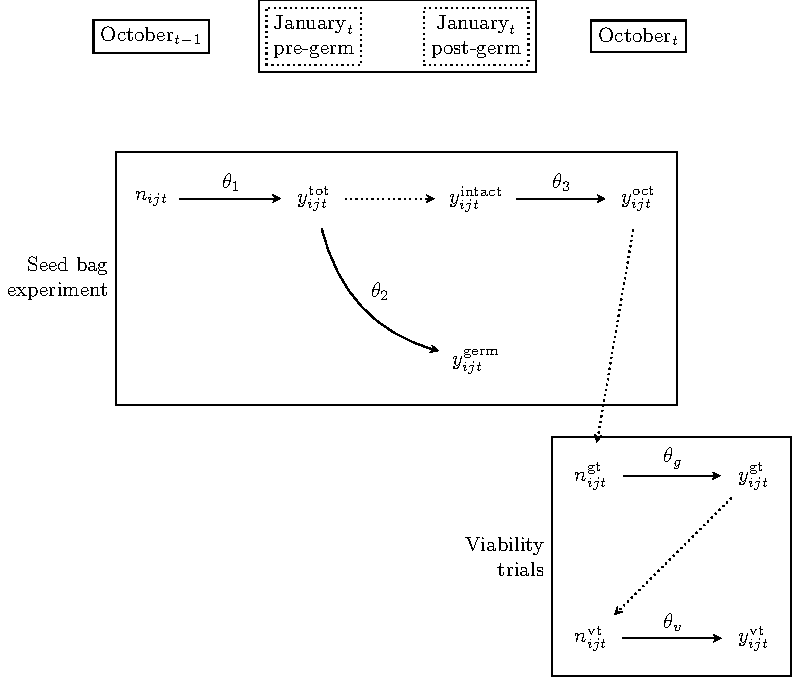
\includegraphics[page=1,width=.9\textwidth]{../../miscellaneous/seed-bag-figure.pdf}  
  \caption{Diagram of data from the seed bag experiments and viability trials. There are two boxes: one for the seed bag experiment and one for the viability trials. In the seed bag experiment, I split January into two steps, one for just before germination and one for just after. Solid arrows represent probabilities estimated with a binomial experiment and are labeled with corresponding parameters. Dotted arrows represent cases where the seeds at the head of the arrow include some, possibly all, seeds at the tail of the arrow.}\label{seedexperiments}
 \label{fig:seedBagDiagram}
\end{figure}

\clearpage
%%%%%%%%%%%%%%%%%%%%%%%%%%%%%%%%%%%%%%%%%%%%%%%%%%%%
% BIBLIOGRAPHY
%%%%%%%%%%%%%%%%%%%%%%%%%%%%%%%%%%%%%%%%%%%%%%%%%%%%
\bibliographystyle{/Users/gregor/Dropbox/bibliography/styleFiles/ecology} 
\bibliography{/Users/gregor/Dropbox/bibliography/chapter-1}

\end{document}